%Je nach dem in welcher Sprache ihr euer Paper schreiben wollt, benutzt bitte entweder den Deutschen-Titel oder den Englischen (einfach aus- bzw. einkommentieren mittels '%')

%Deutsch
\section{Methodischer Ansatz}

%Englisch
%\section{Methodological Approach}

%%ieses Kapitel ist das Herzstück eures Position Papers, wo ihr euren Lösungsansatz beschreibt. Je nach dem in welche Richtung euer Thema geht, kann dieses Kapitel auf unterschiedliche Arten aufgezogen werden. Folgende Informationen könnten (müssen jedoch nicht) Teil dieses Kapitels sein:
%%\begin{itemize}
%%	\item\textbf{Use Case Beschreibung}\\
%%	In den meisten Fällen wird man als Startpunkt einen bestimmten Use Case haben, den man als Beispiel heranzieht bzw. den man im Zuge des Projektes bearbeiten möchte / wird. Der Use Case könnte sogar als Einstiegspunkt in die Thematik dienen, wo man die Problemstellung nochmal bildlich darstellt und auf Basis dessen den Lösungsansatz erklärt bzw. motiviert.
	
%%	Die Use Case Beschreibung soll das \textit{\textbf{"WAS möchte man sich anschauen"}} darstellen und beschreiben.\\
		
%%	\item\textbf{Technische Beschreibung eures Prototypen / eures Demonstrators}\\
%%	Wenn man erklärt hat WAS man sich anschauen möchte, wäre die nächste Frage \textit{\textbf{"WIE möchte man es sich anschauen"}}. Dabei wäre eine technische Beschreibung de Veruchsaufbaus / Demonstrators sehr gut geeignet, wo man motiviert, WIE man vor hat die Problemstellung zu bearbeiten. Dieser Teil könnte sogar auf der Use Case Beschreibung aufbauen und die technische Ausführung des Use Cases erklären. 
	
%%	\item\textbf{Beschreibung was ihr messen / evaluieren / vergleichen / analysieren werdet}\\
%%	Je nach dem in welchem Themengebiet man unterwegs ist und welche Problemstellung man bearbeitet, wird man unterschiedliche methodische Ansätze verwenden können. Hier geht es vor allem darum zu erklären, welchen Ansatz man wählt um die Problemstellung zu bearbeiten und in welcher Art und Weise man vor hat Daten zu sammeln bzw. Ergebnisse zu erzielen, um das Problem zu bearbeiten / zu lösen. Ein wichtiger Aspekt cabei könnte sein welche Metriken man vor hat zu verwenden, damit man Daten sammeln bzw. Ergebnisse erzielen kann, die zeigen, WIE man die Problemstellung tatsächlich löst.
%%\end{itemize}

%%\textbf{VORGABE}: dieses Kapitel soll nicht mehr 3 A4-Seiten benötigen


%%%%%%%%%%%%%%%%%%%%%%%%%%%%%%%%%%%%%%%%%%%%%%%%%%%%%%%%%%%%%%%%%%%%%%%%%%%%%%%%%%%%%%%%%%%%%%%
% hier das erste zusammensammeln an Infos -- NOCH NICHT FERTIG !!
%%%%%%%%%%%%%%%%%%%%%%%%%%%%%%%%%%%%%%%%%%%%%%%%%%%%%%%%%%%%%%%%%%%%%%%%%%%%%%%%%%%%%%%%%%%%%%%

\subsection{Use Case Beschreibung}
Der Use Case fokussiert sich auf die Schaffung eines adaptiven Smart Office für neurodivergente Personen 
(z.B. ADHS, Autismus) und Burnout-Rückkehrer:innen. Ziel ist es, durch Echtzeit-Anpassungen der Arbeitsumgebung sensorische
Überlastung zu reduzieren und produktives Arbeiten zu fördern. Konkret umfasst der Use Case folgende Szenarien:
\begin{itemize}
    \item \textbf{Profilbasierte Anpassung}: Nutzer:innen erstellen individuelle Profile mit Präferenzen für Lichtintensität,
	 Farbtemperatur, Hintergrundgeräusche und visuelle Strukturierung (z.B. Tagesplanvisualisierung).
    \item \textbf{Dynamische Reizsteuerung}: IoT-Sensoren messen Umweltparameter (Licht, Lärm, CO2) und triggern automatische 
	Anpassungen (z.B. Dimmen fluoreszierender Beleuchtung bei ADHS-Profilen).
    \item \textbf{Präventives Stressmanagement}: Ein Dashboard priorisiert Aufgaben, filtert Unterbrechungen und visualisiert 
	Arbeitsabläufe, um Stressquellen für Autist:innen und Burnout gefährdete Personen zu minimieren.
\end{itemize}

\subsection{Technische Umsetzung des Prototyps}
Die Architektur stellt eine Vereinfachung der bestehenden Architektur, welche in \cite{ref01}{Towards a Cloud-Based Smart Office 
Solution for Shared Workplace Individualization} gefunden werden kann dar. Sie baut auf einem AWS-basierten Framework 
(vgl. Abb. \ref{fig:schematic-prototype}) auf und erweitert dieses um zielgruppenspezifische Komponenten:

\begin{figure}[!h]
	\center
	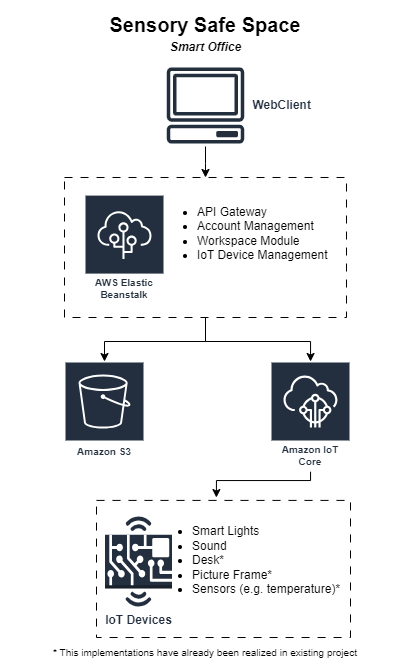
\includegraphics[height=3.5cm]{fig/SchmematicAwsV5-Seite-3.drawio.png}
		\caption{Architektur des Smart-Office-Prototyps}
		\label{fig:schematic-prototype}
\end{figure}

%%%%%%%%%%%%%%%%%%%%%%%%%%%%%%%%%%%%%%%%%%%%%%%%%%%%%%%%%%%%%%%%%%%%%%%%%%%%%%%%%%%%%%%%%%%%%%%
% TODO: Erster Entwurf der Kernkomponenten und Evaluierungsmethoden
%%%%%%%%%%%%%%%%%%%%%%%%%%%%%%%%%%%%%%%%%%%%%%%%%%%%%%%%%%%%%%%%%%%%%%%%%%%%%%%%%%%%%%%%%%%%%%%	

\subsubsection{Kernkomponenten}
*Die Kernkomponenten des Prototyps umfassen AWS-basierte Services, die die grundlegenden Funktionen des Systems bereitstellen.
AWS Elastic Beanstalk dient als Host für die Backend Logik und ....  Das API Gateway dient als Schnittestelle zwischen WebClient 
und IoT-Geräten und verwendet  z.B. Zigbee-API, MQTT, ... * und sorgt für eine reibungslose Kommunikation zwischen den Komponenten.
Die IoT Device Management Komponente sorgt für die Verwaltung der Geräte (z.B. Smart Lights, Desk, Picture Frame), sowie die 
zielgruppenspezifischen Erweiterungen (z.B. Lichtsteuerung, Akustik, Dashboard). Dabei dient Amazon S3 als Speicher für Nutzerdaten
(Opt-in) und Sensorwerte.


\subsubsection{Erweiterungen für Zielgruppen}
Diese Komponenten sind spezifisch für die zielgruppengerichtete Anpassung des Systems dienlich und werden über die 
Kernkomponenten hinaus implementiert. Philips Hue-Lampen (oder sonst iwelche Smart Lights) passen sich via Zigbee-API
an Tageszeit und Nutzerprofile an (z.B. warmes Licht für Autist:innen). Ein Raspberry Pi oder Microcontroller (oder sonstige Hardware)
mit Noise-Cancelling-Software generiert individuell angepasste Soundscapes (z.B. Weißes Rauschen für ADHS-Betroffene).
React-basierte Oberfläche mit drag-and-drop-Tagesplaner und Priorisierungsalgorithmus (Eisenhower-Matrix)....


\subsection{Evaluationsmethoden}

\subsubsection{DELTA Analyse}
Hier soll verglichen werden welche Veränderungen sich von \cite{ref01}{Towards a Cloud-Based Smart Office 
Solution for Shared Workplace Individualization} durch die zielgruppenspezifische Erweriterung ergeben


\subsubsection{Performance-Messung}
Um die Wirksamkeit des Systems zu validieren, werden folgende Metriken und Tools eingesetzt:
AWS CloudWatch überwacht Antwortzeiten der IoT-Geräte (Ziel: <500 ms für Echtzeit-Anpassungen).
Lasttests mit JMeter simulieren bis zu 1.000 gleichzeitige Nutzer:innen


\subsubsection{Usability und Accessibility}
\begin{itemize}
    \item \textbf{WCAG 2.1-Konformität}: Automatisierte Tests mit Axe und WAVE validieren Barrierefreiheit.
  
%%%%%%%%%%%%%%%%%%%%%%%%%%%%%%%%%%%%%%%%%%%%%%%%%%%%%%%%%%%%%%%%%%%%%%%%%%%%%%%%%%%%%%%%%%%%
%% Tools die sich anbieten würden hierfür:
%% https://sparkbox.com/foundry/lighthouse_chrome_website_accessibility_audit_website_accessibility_checker
%%	https://www.deque.com/axe/
%%%%%%%%%%%%%%%%%%%%%%%%%%%%%%%%%%%%%%%%%%%%%%%%%%%%%%%%%%%%%%%%%%%%%%%%%%%%%%%%%%%%%%%%%%%%

vllcht light/Dark mode -- Lichtempfindlichkeit Autist:innen
Generierung eines quantitativen Accessibility-Scores pro Komponente (z.B. 95/100 für das Dashboard) - 
Ein Accessibility-Score ist eine Zahl zwischen 0 und 100, die angibt, wie barrierefrei eine Komponente
 (z.B. ein Button, ein Formular oder das gesamte Dashboard) ist.
 Beispiel:
 95/100: Die Komponente erfüllt fast alle Kriterien, hat aber geringfügige Verbesserungspotenziale.
  70/100: Es gibt deutliche Mängel, die bestimmte Nutzer:innen ausschließen (z.B. fehlende Alt-Texte).

\end{itemize}

Der methodische Ansatz kombiniert technische Agilität (AWS, IoT) mit psychologischer Prävention und ethischer Verantwortung. 
Durch die Integration verschiedener Komponenten aus \cite{ref01}{Towards a Cloud-Based Smart Office Solution for Shared Workplace 
Individualization} und den zielgruppenspezifischen Erweiterungen wird eine intersektionale Plattform geschaffen, die Inklusion 
in der Arbeitswelt neu definieren könnte und die Bedürfnisse neurodivergenter Menschen und Burnout-Rückkehrer:innen berücksichtigt,
um diesen Gruppen ein angemessenes und inklusives Arbeitsumfeld zu schaffen.
